\section{Results}
\label{sec:results}

Results are organised by doctrine clause. Every number cites a gate record by identifier; fail verdicts are reported as registered negatives. Findings F1 to F6 confirm mechanisms; F7 to F9 bound scope.

\subsection{F1: Loadability Replicates and Scales; Pruning Collapses It}
\label{sec:results:loadability}

Instructed loading writes a verbalizable concept code into the band and counts the fraction of prompts on which the concept surfaces in the model's top-5 continuation tokens (hit-rate@5, $n=40$ prompts, shuffled-code null with 200 resamples). On Qwen3-4B the instructed rate is 0.10 against a null of 0.0104 (permutation $p \approx 10^{-4}$, gate L1). On Qwen3.6-27B the rate rises to 0.55 (22 of 40, null 0.068), clearing the registered 0.5 threshold (gate L1b). On Nemotron-Mini-4B, a pruned-and-distilled model, the instructed rate is 0.00, indistinguishable from its null and from an uninstructed control (gate L2). Figure~\ref{fig:loadability} plots all three against their nulls. Loadability is therefore not a generic property of decoder transformers at a given size: it scales with size within a lineage and can be absent at 4B when the training pipeline includes pruning and distillation \cite{Minitron2024}. Band structure itself is present in all three models (CKA band contrast 0.306, 0.269, and 0.137 respectively, gates L1, L1b, L2), so what varies is writability, not banding. A registered reportability metric behaved anomalously in the same experiments, concentrating on the final layers rather than the late third on both Qwen sizes (Spearman $\rho$ of 0.180 at 4B and 0.124 at 27B against a 0.4 threshold); this is recorded as a failed sub-hypothesis in both gates rather than adjusted away.

\begin{figure}[t]
\centering
\resizebox{\columnwidth}{!}{% Auto-generated from committed gate JSONs by generate_figures.py. Do not edit by hand.

\begin{tikzpicture}
\begin{axis}[
  ybar, /pgf/bar width=11pt,
  width=\columnwidth, height=0.62\columnwidth,
  ymin=0, ymax=0.65,
  ylabel={Instructed hit-rate@5},
  symbolic x coords={Qwen3-4B,Qwen3.6-27B,Nemotron-Mini-4B},
  xtick=data, x tick label style={font=\scriptsize},
  ytick={0,0.1,0.2,0.3,0.4,0.5,0.6},
  ylabel style={font=\small}, tick label style={font=\scriptsize},
  legend style={font=\scriptsize, at={(0.03,0.97)}, anchor=north west, draw=none, fill=none},
  ymajorgrids, grid style={gray!25},
  axis line style={gray!60},
]
\addplot+[fill=blue!55, draw=blue!70!black] coordinates {(Qwen3-4B,0.1) (Qwen3.6-27B,0.55) (Nemotron-Mini-4B,0.0)};
\addplot+[fill=gray!35, draw=gray!60, postaction={pattern=north east lines, pattern color=gray!70}] coordinates {(Qwen3-4B,0.010375) (Qwen3.6-27B,0.06824999999999999) (Nemotron-Mini-4B,0.0)};
\addlegendentry{instructed write}
\addlegendentry{shuffled-code null}
\draw[dashed, red!70] (rel axis cs:0,0.769) -- (rel axis cs:1,0.769) node[pos=0.98, above left, font=\tiny, red!70] {registered threshold 0.5};
\end{axis}
\end{tikzpicture}
}
\caption{Instructed loadability across plants (gates L1, L1b, L2). Bars give instructed hit-rate@5; hatched bars give the shuffled-code null. The 27B model clears the registered 0.5 threshold; the pruned-and-distilled twin shows no instructed loading at all.}
\label{fig:loadability}
\end{figure}

\subsection{F2: Band Content Is Legible Only to a Band-Targeted Lens, and the Gradient Is Model-Intrinsic}
\label{sec:results:articulation}

On the twin whose instructed loading reads as absent, a lens fitted to final output logits reads the band as empty across seven instructed concepts (0.00), while a lens targeted at the band's own exit (layer 26) reads directed loading at 0.20 against a null of 0.023 (gate L2b). The same articulation-depth gradient, read-out negentropy rising through the band, appears on every plant tested. A registered null experiment addresses the concern that the gradient is an artifact of lens construction: the gradient survives under a logit-lens read-out that involves no fitted transport, with Spearman $\rho = 0.607$ against $\rho = 0.639$ for the Jacobian lens, both at permutation $p = 2 \times 10^{-4}$ (gate L7; Figure~\ref{fig:articulation}). The gradient is a property of the model's residual stream. The engineering consequence is direct: readback verification must use band-targeted lenses, and final-lens analyses of band interventions produce false negatives.

\begin{figure}[t]
\centering
\resizebox{\columnwidth}{!}{% Auto-generated from committed gate JSONs by generate_figures.py. Do not edit by hand.

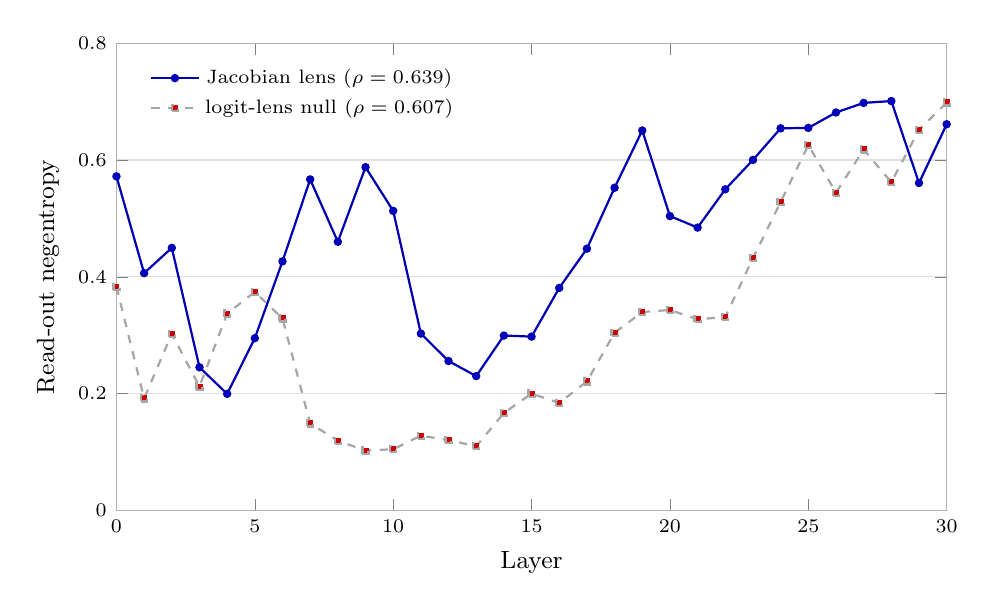
\begin{tikzpicture}
\begin{axis}[
  width=\columnwidth, height=0.62\columnwidth,
  xlabel={Layer}, ylabel={Read-out negentropy},
  xmin=0, xmax=30, ymin=0, ymax=0.8,
  label style={font=\small}, tick label style={font=\scriptsize},
  legend style={font=\scriptsize, at={(0.03,0.97)}, anchor=north west, draw=none, fill=none},
  ymajorgrids, grid style={gray!25}, axis line style={gray!60},
]
\addplot+[mark=*, mark size=1.1pt, blue!70!black, thick] coordinates {(0,0.572) (1,0.4063) (2,0.4496) (3,0.2452) (4,0.1997) (5,0.295) (6,0.4265) (7,0.5668) (8,0.46) (9,0.5877) (10,0.5129) (11,0.3029) (12,0.2559) (13,0.2301) (14,0.2995) (15,0.2977) (16,0.381) (17,0.4482) (18,0.5525) (19,0.6505) (20,0.504) (21,0.4843) (22,0.5498) (23,0.6001) (24,0.6542) (25,0.6549) (26,0.6813) (27,0.6977) (28,0.7009) (29,0.5606) (30,0.6612)};
\addplot+[mark=square*, mark size=1.1pt, gray!70, thick, dashed] coordinates {(0,0.3831) (1,0.1919) (2,0.3024) (3,0.2122) (4,0.3371) (5,0.3742) (6,0.3288) (7,0.1491) (8,0.1195) (9,0.1026) (10,0.1049) (11,0.128) (12,0.1207) (13,0.11) (14,0.1669) (15,0.2001) (16,0.1841) (17,0.2209) (18,0.3042) (19,0.3398) (20,0.3433) (21,0.3274) (22,0.331) (23,0.4321) (24,0.5279) (25,0.6256) (26,0.544) (27,0.6179) (28,0.5619) (29,0.6515) (30,0.6985)};
\addlegendentry{Jacobian lens ($\rho=0.639$)}
\addlegendentry{logit-lens null ($\rho=0.607$)}
\end{axis}
\end{tikzpicture}
}
\caption{Per-layer read-out negentropy for the fitted Jacobian lens and for a logit-lens null with no fitted transport (gate L7). Both read-outs recover the articulation gradient with permutation $p=2\times10^{-4}$, establishing the gradient as model-intrinsic.}
\label{fig:articulation}
\end{figure}

\subsection{F3: Uncapped Writing Steers but Destroys Freedom; the Budget Binds}
\label{sec:results:budget}

Unrestricted band writing lifts concept surfacing to 0.40 (baseline 0.00) but costs $-2.081$ nats of trajectory entropy, four times the registered budget (gate L3). The gate's failure taxonomy attributes 20 of the 40 write attempts to freedom-criterion rejection, 14 to uptake failure, and 2 to write-quality failure, identifying freedom cost as the binding constraint. Decomposition across gates L4 and L4b shows the at-position cost of a single write is large and decoding-independent (approximately $-2$ nats at the write position), while the trajectory-average cost is regime-dependent ($+0.82$ nats greedy, $-0.13$ sampling); the budget currency was registered accordingly (Section~\ref{sec:doctrine:budget}). These two gates are registered negatives that define the constraint the remaining experiments must satisfy.

\subsection{F4: Timing Is the Mechanism; the Flash Variant Failed and Was Revised}
\label{sec:results:timing}

The first timing experiment failed its registered criterion: gated lift 0.175 against a 0.2 threshold, with no advantage over schedule or prefill controls (gate L4). Its successor, with corrected gating, passed: entropy-gated writes reach lift 0.40 at trajectory cost $-0.127$ nats using approximately 9.85 writes per generation, against 0.20 for a single prefill write (gate L4b), the programme's first interventional pass. The threshold $\tau$ is not delicate: six of six runs pass across the P40, P60, and P80 entropy percentiles at two seeds, with lift 0.35 to 0.40 and in-budget entropy deltas throughout (gate L5). Timing beats rate: at matched write budgets, entropy-gated placement (lift 0.40 at 7.15 writes per generation) exceeds a rate-matched schedule (0.225 at 5.0) and prefill (0.20), so when to write matters more than how often (gate L6). The literal flash reading of the timing clause, gating on commitment onsets, adds nothing over prefill (0.20 versus 0.30 for uncommitted-moment gating, gate L9); the revised uncommitted-moment form wins at all three seeds tested (advantages of 0.05 to 0.10, gate L12). The doctrine's timing clause survives in revised form, and the revision is documented in the ledger rather than presented as the original hypothesis.

\subsection{F5: The Core Claim at Six Independent-Stream Seeds}
\label{sec:results:core}

An adversarial review of the early sampling estimates uncovered that a single per-run seed had correlated all generations within an arm, shrinking the effective sample size (gate L9, the stream fix; Section~\ref{sec:setup}). All headline claims were therefore restated on independent streams. The core claim, entropy-gated band writes steer within the freedom budget, holds at all six registered seeds, with gated lift 0.30 to 0.35 and trajectory entropy deltas between $-0.006$ and $+0.246$ nats, all inside the cap (gate L11; Table~\ref{tab:core}; Figure~\ref{fig:core}). The advantage over prefill is positive at every seed (mean $+0.100$, range $+0.075$ to $+0.125$), giving a one-sided sign-test $p = 1/2^6 = 0.0156$; its magnitude, however, clears the registered 0.1 margin at only three of six seeds, and an earlier three-seed confirmation had already split the same way (budget claim 3 of 3, margin claim 1 of 3, gate L6 confirm). The claim supported by the evidence is therefore direction, not size: gating always helps, by a margin near 0.1. Steering is also operationally free in throughput terms: steered arms decode at 24.8 to 25.0 tokens per second against a 19.7 baseline on the shared node, so write count imposes no serving cost at this scale (gate L9 write-cost).

\begin{table}[t]
\caption{Core claim at six independent-stream seeds (gate L11). Lift is concept hit-rate@5 over baseline; advantage is gated minus prefill; $\Delta H$ is trajectory-average entropy change (budget $\pm0.5$ nats). Sign consistency 6/6, one-sided $p=0.0156$.}
\label{tab:core}
\vskip 0.1in
\centering
{\small
\begin{tabular}{lccc}
\toprule
\textbf{Seed} & \textbf{Gated lift} & \textbf{Advantage} & $\bm{\Delta H}$ \textbf{(nats)} \\
\midrule
42    & 0.30 & $+0.075$ & $+0.112$ \\
123   & 0.35 & $+0.125$ & $+0.246$ \\
777   & 0.35 & $+0.075$ & $+0.109$ \\
2024  & 0.35 & $+0.125$ & $-0.006$ \\
31415 & 0.35 & $+0.100$ & $+0.094$ \\
999   & 0.35 & $+0.100$ & $+0.149$ \\
\midrule
mean  & 0.342 & $+0.100$ & $+0.117$ \\
\bottomrule
\end{tabular}}
\end{table}

\begin{figure}[t]
\centering
\resizebox{\columnwidth}{!}{% Auto-generated from committed gate JSONs by generate_figures.py. Do not edit by hand.

\begin{tikzpicture}
\begin{groupplot}[
  group style={group size=2 by 1, horizontal sep=34pt},
  width=0.56\columnwidth, height=0.56\columnwidth,
  symbolic x coords={42,123,777,2024,31415,999},
  xtick=data, xlabel={seed}, x tick label style={rotate=45, anchor=east},
  label style={font=\scriptsize}, tick label style={font=\scriptsize},
  ymajorgrids, grid style={gray!25}, axis line style={gray!60},
]
\nextgroupplot[ybar, /pgf/bar width=4.5pt, ymin=0, ymax=0.45, ylabel={lift},
  legend style={font=\tiny, at={(0.02,0.98)}, anchor=north west, draw=none, fill=none}]
\addplot+[fill=blue!55, draw=blue!70!black] coordinates {(42,0.3) (123,0.35) (777,0.35) (2024,0.35) (31415,0.35) (999,0.35)};
\addplot+[fill=orange!55, draw=orange!70!black] coordinates {(42,0.075) (123,0.125) (777,0.075) (2024,0.125) (31415,0.1) (999,0.1)};
\addlegendentry{gated lift}
\addlegendentry{advantage over prefill}
\draw[dashed, red!70] (rel axis cs:0,0.444) -- (rel axis cs:1,0.444);
\nextgroupplot[ybar, /pgf/bar width=6pt, ymin=-0.55, ymax=0.55, ylabel={$\Delta H$ (nats)}]
\addplot+[fill=teal!45, draw=teal!70!black] coordinates {(42,0.1118) (123,0.2457) (777,0.1087) (2024,-0.006) (31415,0.0936) (999,0.1485)};
\draw[dashed, gray!80] (rel axis cs:0,0.954) -- (rel axis cs:1,0.954);
\draw[dashed, gray!80] (rel axis cs:0,0.045) -- (rel axis cs:1,0.045);
\end{groupplot}
\end{tikzpicture}
}
\caption{The core claim at six independent-stream seeds (gate L11). Left: gated lift and advantage over prefill per seed; the dashed line marks the registered 0.2 lift threshold. Right: trajectory entropy deltas, all within the $\pm0.5$-nat budget (dashed lines).}
\label{fig:core}
\end{figure}

\subsection{F6a: Dose Response by Timing Arm, with a Documented Supersession}
\label{sec:results:dose}

The canonical dose grid (gate L18, three amplitudes, clean streams) is shown in Figure~\ref{fig:timing}. Continuous writing reaches the highest surface lift (0.45 to 0.50) at 24.7 to 29 writes per generation; entropy-gated writing reaches 0.275 to 0.30 at 8.4 to 9.0 writes; rate-matched and prefill controls sit at 0.15 to 0.225. All gated points are within budget. An earlier version of this grid (gate L8) predated the stream fix and ran approximately 0.1 high at the gated points; the supersession is formal, confirmed at three seeds and two amplitudes with all six per-seed offsets negative (mean $-0.108$ at $\alpha=0.02$ and $-0.067$ at $\alpha=0.1$, gate L19), and the superseded gate remains in the ledger with its status marked.

\begin{figure}[t]
\centering
\resizebox{\columnwidth}{!}{% Auto-generated from committed gate JSONs by generate_figures.py. Do not edit by hand.

\begin{tikzpicture}
\begin{groupplot}[
  group style={group size=2 by 1, horizontal sep=32pt},
  width=0.56\columnwidth, height=0.56\columnwidth,
  ybar, /pgf/bar width=3.4pt,
  symbolic x coords={0.02,0.05,0.1},
  xtick=data, xlabel={write amplitude $\alpha$},
  label style={font=\scriptsize}, tick label style={font=\scriptsize},
  ymajorgrids, grid style={gray!25}, axis line style={gray!60},
]
\nextgroupplot[ylabel={concept surface lift}, ymin=0, ymax=0.55,
  legend style={font=\tiny, at={(0.02,0.98)}, anchor=north west, draw=none, fill=none, legend columns=1}]
\addplot+[fill=red!50, draw=red!70!black] coordinates {(0.02,0.475) (0.05,0.45) (0.1,0.5)};
\addplot+[fill=blue!55, draw=blue!70!black] coordinates {(0.02,0.275) (0.05,0.275) (0.1,0.3)};
\addplot+[fill=teal!45, draw=teal!70!black] coordinates {(0.02,0.175) (0.05,0.175) (0.1,0.225)};
\addplot+[fill=gray!35, draw=gray!60] coordinates {(0.02,0.175) (0.05,0.15) (0.1,0.2)};
\addlegendentry{continuous}
\addlegendentry{entropy-gated}
\addlegendentry{rate-matched}
\addlegendentry{prefill}
\nextgroupplot[ylabel={writes per generation}, ymin=0, ymax=32]
\addplot+[fill=red!50, draw=red!70!black] coordinates {(0.02,28.95) (0.05,24.73) (0.1,27.23)};
\addplot+[fill=blue!55, draw=blue!70!black] coordinates {(0.02,8.4) (0.05,8.97) (0.1,8.93)};
\addplot+[fill=teal!45, draw=teal!70!black] coordinates {(0.02,6.38) (0.05,7.5) (0.1,7.42)};
\addplot+[fill=gray!35, draw=gray!60] coordinates {(0.02,1.0) (0.05,1.0) (0.1,1.0)};
\end{groupplot}
\end{tikzpicture}
}
\caption{Timing arms across write amplitude on Nemotron-Mini-4B, clean streams (gates L18). Left: concept surface lift; right: writes per generation. Entropy-gated writing obtains roughly 60\,\% of the continuous arm's lift at a third of its writes, within budget; the continuous arm's raw-lift dominance is quantified further in Section~\ref{sec:results:l21}.}
\label{fig:timing}
\end{figure}

\subsection{F6b: The Calibration Recipe Transfers Across Plants; Geometry Does Not}
\label{sec:results:transfer}

Transplanting the working configuration from Nemotron-Mini-4B to Qwen3-4B unchanged fails: gated lift 0.05, prefill 0.00 (gate L10). The diagnosis is quantitative: the target-layer Jacobian transports on Qwen3-4B are roughly ten times weaker than on the donor, so the same amplitude under-drives the band. Site sweeps eliminate layer choice as the blocker (all probed sites read 0.00 under borrowed amplitude, gate L13 probes). The recipe that transfers sets amplitude inversely proportional to lens transport strength: at three times the donor amplitude, Qwen3-4B reaches gated lift 0.40 against prefill 0.175 (gate L13), the dose curve is strictly monotone over a four-point amplitude grid (0.05, 0.20, 0.40, 0.775 at $\alpha$ from 0.1 to 0.45, gate L14), the recipe holds at four seeds (gated 0.325 to 0.475, prefill 0.075 to 0.175, all in budget, gate L14 multiseed; Figure~\ref{fig:recipe}), and per-seed monotonicity replicates at two further seeds (gate L15). On the donor side, a fine amplitude grid finds the same law at one-tenth the scale, rising from 0.025 at $\alpha=0.002$ to saturation near 0.275 at $\alpha=0.01$ (gate L16). Together the two plants trace a dose law spanning roughly 1.5 orders of amplitude magnitude (Figure~\ref{fig:scaling}). The gate discloses the limits: the two-plant statement is ordering and saturation consistency at screen tier, the within-plant monotone law is the confirmed component, and the donor curve's flat first pair carries no dose signal (gate L15 disclosures).

\begin{figure}[t]
\centering
\resizebox{\columnwidth}{!}{% Auto-generated from committed gate JSONs by generate_figures.py. Do not edit by hand.

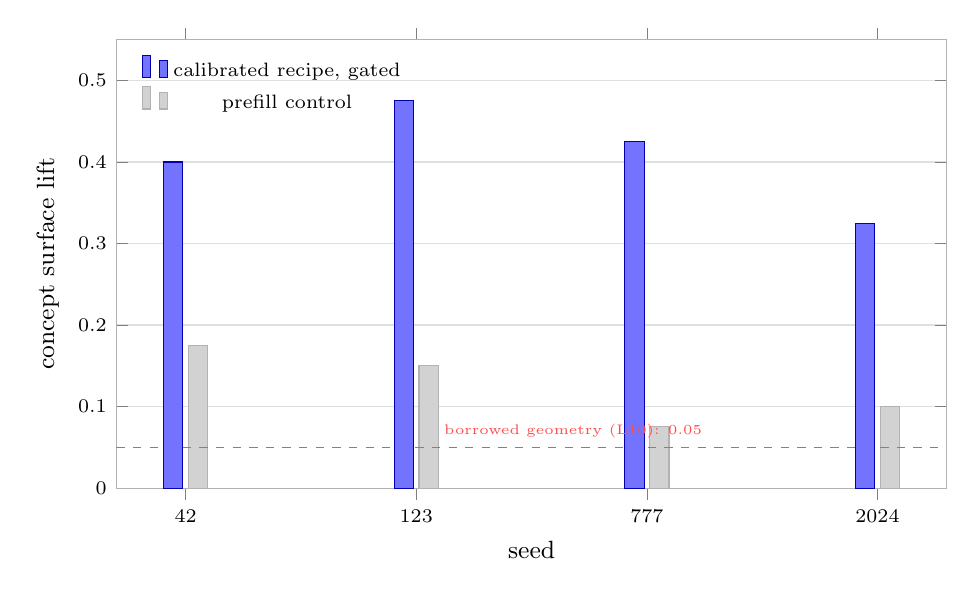
\begin{tikzpicture}
\begin{axis}[
  ybar, /pgf/bar width=7pt,
  width=\columnwidth, height=0.6\columnwidth,
  symbolic x coords={42,123,777,2024},
  xtick=data, xlabel={seed},
  ymin=0, ymax=0.55, ylabel={concept surface lift},
  label style={font=\small}, tick label style={font=\scriptsize},
  legend style={font=\scriptsize, at={(0.02,0.98)}, anchor=north west, draw=none, fill=none},
  ymajorgrids, grid style={gray!25}, axis line style={gray!60},
]
\addplot+[fill=blue!55, draw=blue!70!black] coordinates {(42,0.4) (123,0.475) (777,0.425) (2024,0.325)};
\addplot+[fill=gray!35, draw=gray!60] coordinates {(42,0.175) (123,0.15) (777,0.075) (2024,0.1)};
\addlegendentry{calibrated recipe, gated}
\addlegendentry{prefill control}
\draw[dashed, red!70] (rel axis cs:0,0.0909) -- (rel axis cs:1,0.0909)
  node[pos=0.55, above, font=\tiny, red!70] {borrowed geometry (L10): 0.05};
\end{axis}
\end{tikzpicture}
}
\caption{Recipe transfer to Qwen3-4B at four seeds (gate L14 multiseed): calibrated-amplitude gated writes against prefill controls. The dashed line marks the lift obtained by transplanting the donor configuration without calibration (0.05, gate L10).}
\label{fig:recipe}
\end{figure}

\begin{figure}[t]
\centering
\resizebox{\columnwidth}{!}{% Auto-generated from committed gate JSONs by generate_figures.py. Do not edit by hand.

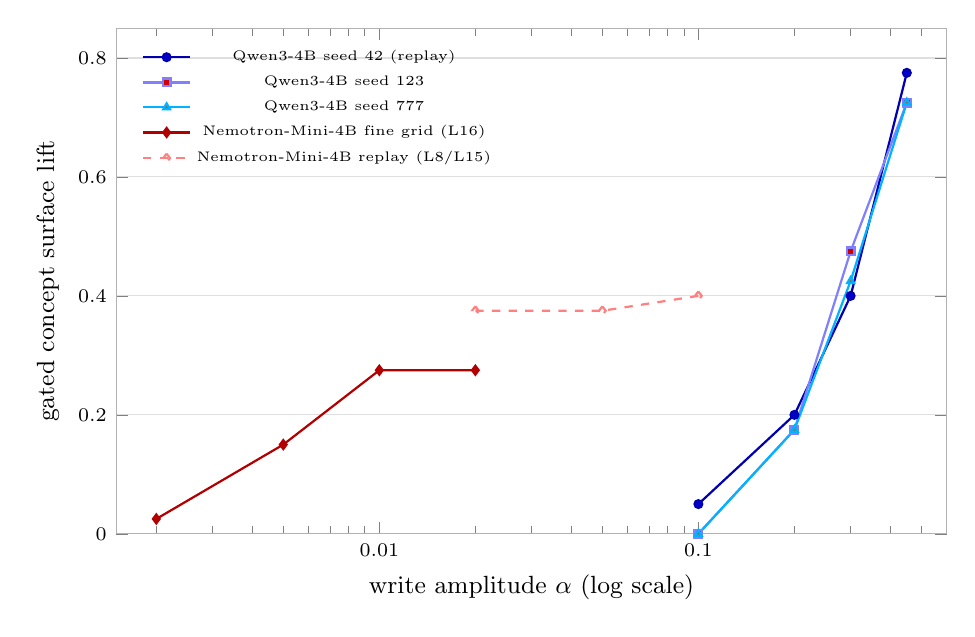
\begin{tikzpicture}
\begin{axis}[
  width=\columnwidth, height=0.66\columnwidth,
  xmode=log, log ticks with fixed point,
  xlabel={write amplitude $\alpha$ (log scale)}, ylabel={gated concept surface lift},
  xmin=0.0015, xmax=0.6, ymin=0, ymax=0.85,
  label style={font=\small}, tick label style={font=\scriptsize},
  legend style={font=\tiny, at={(0.02,0.98)}, anchor=north west, draw=none, fill=none},
  ymajorgrids, grid style={gray!25}, axis line style={gray!60},
]
\addplot+[blue!70!black, mark=*, thick, mark size=1.4pt] coordinates {(0.1,0.05) (0.2,0.2) (0.3,0.4) (0.45,0.775)};
\addlegendentry{Qwen3-4B seed 42 (replay)}
\addplot+[blue!50, mark=square*, thick, mark size=1.4pt] coordinates {(0.1,0.0) (0.2,0.175) (0.3,0.475) (0.45,0.725)};
\addlegendentry{Qwen3-4B seed 123}
\addplot+[blue!30!cyan, mark=triangle*, thick, mark size=1.4pt] coordinates {(0.1,0.0) (0.2,0.175) (0.3,0.425) (0.45,0.725)};
\addlegendentry{Qwen3-4B seed 777}
\addplot+[red!70!black, thick, mark=diamond*, mark size=1.6pt] coordinates {(0.002,0.025) (0.005,0.15) (0.01,0.275) (0.02,0.275)};
\addlegendentry{Nemotron-Mini-4B fine grid (L16)}
\addplot+[red!50, thick, dashed, mark=diamond, mark size=1.6pt] coordinates {(0.02,0.375) (0.05,0.375) (0.1,0.4)};
\addlegendentry{Nemotron-Mini-4B replay (L8/L15)}
\end{axis}
\end{tikzpicture}
}
\caption{Two-plant amplitude law (gates L14, L15, L16, L8 replay). Gated lift against write amplitude on a log axis: Qwen3-4B at three seeds (blue), Nemotron-Mini-4B fine grid (red, solid) and replayed working points (red, dashed). The working amplitudes differ by an order of magnitude in the direction predicted by inverse lens transport strength.}
\label{fig:scaling}
\end{figure}

\subsection{F6c: Readback Tracks Behaviour at Screen Tier; Pooled Generalisation Fails}
\label{sec:results:readback}

The verification clause requires that band readback predict behavioural uptake. On the development corpus, the best readback setting reaches balanced accuracy 0.684 (true-positive rate 0.833, true-negative rate 0.536, $n=40$); the gate disclosal notes that 36 settings were swept, the maximum is reported, and no multiple-comparison correction was applied (gate L14 readback, screen-exploratory). On a held-out corpus with the setting frozen, balanced accuracy is 0.637 against a registered 0.6 threshold, with the margin inside the binomial confidence interval; the same held-out run's steering lift failed its own budget-gate criterion, so lift is corpus-dependent (gate L15 readback, downgraded from confirm to screen by adversarial review). Pooled across three corpus styles ($n=120$), balanced accuracy falls to 0.590, below threshold, and is recorded as a negative exploratory result (gate L16). The verification clause is therefore supported at screen tier on matched corpora and unproven in pooled generalisation.

\subsection{F6d: Corpus Robustness Is an Amplitude Question}
\label{sec:results:corpus}

Gated steering passes on two of three corpus styles at the working amplitude (narrative-past 0.25, descriptive-scene 0.30, held-out replay 0.15 against a 0.2 bar, gate L16). A seed-variance audit then found the narrative corpus seed-fragile at that amplitude (0.25, 0.075, 0.10 across three seeds) while the descriptive corpus is seed-robust (0.30, 0.20, 0.25), a self-audit fail recorded at 2 of 4 registered cells (gate L17). Doubling the amplitude repairs the fragile corpus at all three seeds (0.425, 0.275, 0.225, one margin thin at 0.225 against 0.2, gate L18), and both corpora approximately double their lift under the amplitude increase (0.175 to 0.325 and 0.275 to 0.55, with one registered per-seed margin failing at 0.025 against 0.05, gate L19). The supported statement is that corpus difficulty loads on the amplitude axis, held at screen tier with one disclosed margin failure; a stronger corpus-amplitude law is registered as open.

\subsection{F7: An Untrained Associative-Memory Write Path Matches the Analytic Path}
\label{sec:results:bridge}

The doctrine's write direction $J^{\top}u$ is analytic. A biologically-motivated alternative routes the write through recall from a modern-Hopfield associative store \cite{Ramsauer2021}, the CittaStore of the author's predictive-world-model stack. Integrated end-to-end and run cold, with no patterns stored and no training, the store's recall direction steers within budget on all three seeds (lifts 0.4445, 0.5556, 0.4445, gate L20), and matches the analytic path exactly on two seeds (gaps 0.0000) while differing by a single concept-hit on the third (0.4445 against 0.3334, a gap of 0.1111 against a 0.05 equivalence criterion, in the cold store's favour, at the metric's 1/9 quantisation). The registered equivalence verdict is fail-on-margin at 2 of 3. The store is untrained, so the result is an integration proof that the associative write pathway is live and dimensionally compatible, not evidence that a trained store beats the analytic baseline. Whether training the store improves on cold initialisation is registered as open. Figure~\ref{fig:l20} plots both arms.

\begin{figure}[t]
\centering
\resizebox{\columnwidth}{!}{% Auto-generated from committed gate JSONs by generate_figures.py. Do not edit by hand.

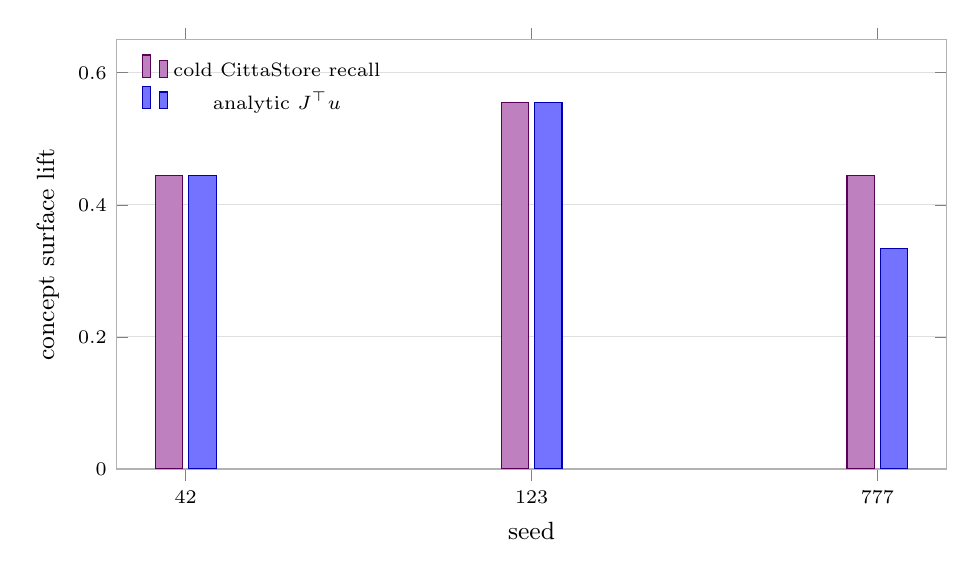
\begin{tikzpicture}
\begin{axis}[
  ybar, /pgf/bar width=10pt,
  width=\columnwidth, height=0.58\columnwidth,
  symbolic x coords={42,123,777},
  xtick=data, xlabel={seed},
  ymin=0, ymax=0.65, ylabel={concept surface lift},
  label style={font=\small}, tick label style={font=\scriptsize},
  legend style={font=\scriptsize, at={(0.02,0.98)}, anchor=north west, draw=none, fill=none},
  ymajorgrids, grid style={gray!25}, axis line style={gray!60},
]
\addplot+[fill=violet!50, draw=violet!70!black] coordinates {(42,0.4445) (123,0.5556) (777,0.4445)};
\addplot+[fill=blue!55, draw=blue!70!black] coordinates {(42,0.4445) (123,0.5556) (777,0.3334)};
\addlegendentry{cold CittaStore recall}
\addlegendentry{analytic $J^{\top}u$}
\end{axis}
\end{tikzpicture}
}
\caption{Cold associative-store recall against the analytic write direction at three seeds (gate L20). Two seeds match exactly; the third differs by one concept-hit (the metric's quantisation unit) in the cold store's favour.}
\label{fig:l20}
\end{figure}

\subsection{F8: Gated Steering Is a Legibility Mechanism, Not a Throughput Maximiser}
\label{sec:results:l21}

A five-arm comparative evaluation on Qwen3-4B ($n=25$ per arm per seed, three seeds) measures concept surface rate (CSR), a heuristic attack-success proxy (ASR), refusal rate, and entropy cost (gates L21 baselines; Table~\ref{tab:l21}; Figure~\ref{fig:l21}). Continuous flooding surfaces concepts at 0.96; entropy-gated and prefill writes surface at 0.16; a logit-bias arm with no layer or timing structure reaches 0.40. Entropy costs are small in all arms ($-0.043$ to $+0.073$ nats), so at matched, negligible entropy cost the continuous arm outperforms the gated arm on raw throughput by a factor of six. The gated arm's registered CSR criterion (at least 0.2) fails at all three seeds, and the verdicts are recorded as fails. The reading consistent with the full ledger is that gating purchases verified, budgeted, moment-targeted content placement rather than maximal surfacing; where raw surfacing is the goal, flooding a 4B model is easy and needs no doctrine. This reframes the doctrine's value as internal-model transparency under constraint, and Section~\ref{sec:discussion} develops the point.

\begin{table}[t]
\caption{Comparative evaluation on Qwen3-4B (gates L21 baselines, mean of seeds 42, 123, 777; $n=25$ per arm per seed). CSR is concept surface rate; ASR is a heuristic attack-success proxy on the same prompt set; $\Delta H$ is mean entropy cost in nats. Per-seed values are identical to three decimals across seeds.}
\label{tab:l21}
\vskip 0.1in
\centering
{\small
\begin{tabular}{lcccc}
\toprule
\textbf{Arm} & \textbf{CSR} & \textbf{ASR} & \textbf{Refusal} & $\bm{\Delta H}$ \\
\midrule
baseline       & 0.000 & 0.800 & 0.200 & $+0.000$ \\
prefill        & 0.160 & 1.000 & 0.000 & $-0.020$ \\
entropy-gated  & 0.160 & 1.000 & 0.000 & $-0.020$ \\
logit bias     & 0.400 & 0.800 & 0.200 & $-0.043$ \\
continuous     & 0.960 & 1.000 & 0.000 & $+0.073$ \\
\bottomrule
\end{tabular}}
\end{table}

\begin{figure}[t]
\centering
\resizebox{\columnwidth}{!}{% Auto-generated from committed gate JSONs by generate_figures.py. Do not edit by hand.

\begin{tikzpicture}
\begin{groupplot}[
  group style={group size=2 by 1, horizontal sep=34pt},
  width=0.56\columnwidth, height=0.56\columnwidth,
  ybar, /pgf/bar width=7pt,
  symbolic x coords={baseline,prefill,entropy-gated,logit bias,continuous},
  xtick=data, x tick label style={rotate=45, anchor=east, font=\tiny},
  label style={font=\scriptsize}, tick label style={font=\scriptsize},
  ymajorgrids, grid style={gray!25}, axis line style={gray!60},
]
\nextgroupplot[ylabel={concept surface rate}, ymin=0, ymax=1.05]
\addplot+[fill=blue!55, draw=blue!70!black] coordinates {(baseline,0.000) (prefill,0.160) (entropy-gated,0.160) (logit bias,0.400) (continuous,0.960)};
\nextgroupplot[ylabel={mean $\Delta H$ (nats)}, ymin=-0.1, ymax=0.1]
\addplot+[fill=teal!45, draw=teal!70!black] coordinates {(baseline,0.000) (prefill,-0.020) (entropy-gated,-0.020) (logit bias,-0.043) (continuous,0.073)};
\end{groupplot}
\end{tikzpicture}
}
\caption{Comparative evaluation arms (gates L21 baselines, three-seed means). Left: concept surface rate; right: mean entropy cost. Continuous flooding dominates raw surfacing at negligible entropy cost; the gated arm's value is verified placement, not throughput.}
\label{fig:l21}
\end{figure}

\subsection{F9: Naive Contrastive Directions Do Not Improve Alignment on an Aligned Model}
\label{sec:results:alignment}

Two registered experiments test whether contrastive activation directions \cite{Rimsky2024,Zou2023RepE} improve safety-relevant behaviour on the already-aligned Qwen3-4B instruct model. A refusal direction extracted from labelled harmful and benign pairs and applied at the working site leaves attack success on an AdvBench subset \cite{Zou2023AdvBench} unchanged: ASR 0.250 with and without steering, refusal rate 0.750 in both arms ($n=20$, gate L21 jailbreak, registered fail). A truthfulness direction extracted from TruthfulQA contrasts \cite{Lin2022} fails its registered improvement criterion, with the gate recording identical heuristic scores in both arms ($n=15$, gate L21 truthful, registered fail). The gates disclose their limits: heuristic pattern-based metrics rather than judge models, single-seed direction extraction, and small subsets. Within those limits the result is consistent with the direction-structure analysis of the author's refusal-symmetry work \cite{Sathish2026Refusal} and with evidence that refusal behaviour, while direction-mediated, is not improved by naive single-direction addition on models whose alignment margin is already consolidated \cite{Arditi2024}. Alignment gains at the activation level are not an automatic dividend of naive workspace steering. Finding~F12 shows that the same activation signal, used for input-conditioned recognition rather than blanket addition, does provide a usable defence on some models.

\subsection{F10: Band-Targeted Reading Is Twice as Sensitive as the Final-Target Baseline at Subtle Doses}
\label{sec:results:baseline}

A head-to-head benchmark compares the paper's band-targeted lens against the Jacobian-lens final-target baseline as reading instruments applied to the same deterministic writes, on a fixed grid of ten concepts by eight stubs ($n=80$ paired observations, exact McNemar test, since a deterministic forward pass cannot be reseeded; gate L22, consolidated from committed sub-gates by a recomputation script). Across a write-dose floor sweep (Figure~\ref{fig:lens_baseline}) the two instruments are indistinguishable at doses too small to load the band (both 0.00 at $\alpha=0.02$, both 0.025 at $\alpha=0.05$), then separate sharply at $\alpha=0.1$, where the band-targeted lens detects on 0.475 of pairs against 0.2375 for the final-target lens, a gap of $+0.2375$ with 20 band-only detections against one final-only ($p=2.1\times10^{-5}$). At the saturating dose $\alpha=0.3$ both instruments approach ceiling (band 1.00, final 0.95, gap $+0.05$, $p=0.125$). The registered gap criterion of at least 0.3 is missed by 0.0625, so the verdict is fail-on-margin, and the strong-form necessity claim (that band content is wholly invisible to a final-target lens) is withdrawn under its own falsifier, since the final-target lens does recover most content once the write saturates. The supported statement is that band-targeted reading is roughly twice as sensitive at subtle, budget-respecting doses, with the direction decisive at $p=2.1\times10^{-5}$, and that the two instruments converge only when the intervention is driven hard enough to be detectable by any reasonable readout.

\begin{figure}[t]
\centering
\resizebox{\columnwidth}{!}{% Auto-generated from committed gate JSONs by generate_figures.py. Do not edit by hand.

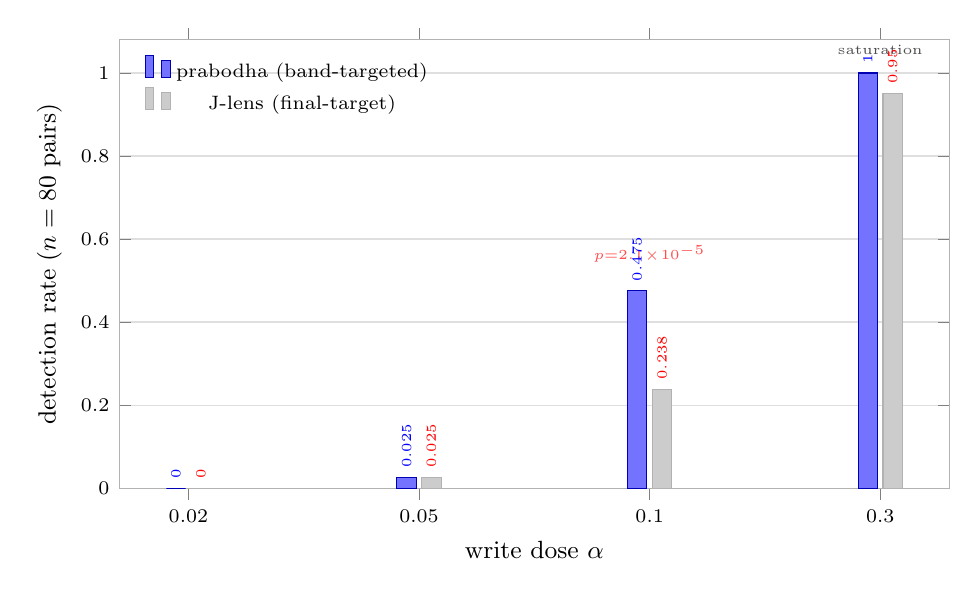
\begin{tikzpicture}
\begin{axis}[
  ybar, /pgf/bar width=7pt,
  width=\columnwidth, height=0.6\columnwidth,
  symbolic x coords={0.02,0.05,0.1,0.3},
  xtick=data, xlabel={write dose $\alpha$},
  ymin=0, ymax=1.08, ylabel={detection rate ($n=80$ pairs)},
  label style={font=\small}, tick label style={font=\scriptsize},
  legend style={font=\scriptsize, at={(0.02,0.98)}, anchor=north west, draw=none, fill=none},
  ymajorgrids, grid style={gray!25}, axis line style={gray!60},
  nodes near coords, nodes near coords style={font=\tiny, /pgf/number format/fixed, /pgf/number format/precision=3},
  every node near coord/.append style={rotate=90, anchor=west},
]
\addplot+[fill=blue!55, draw=blue!70!black] coordinates {(0.02,0.0) (0.05,0.025) (0.1,0.475) (0.3,1.0)};
\addplot+[fill=gray!40, draw=gray!60] coordinates {(0.02,0.0) (0.05,0.025) (0.1,0.2375) (0.3,0.95)};
\addlegendentry{prabodha (band-targeted)}
\addlegendentry{J-lens (final-target)}
\node[font=\tiny, red!70, anchor=south] at (axis cs:0.1,0.52) {$p{=}2.1\!\times\!10^{-5}$};
\node[font=\tiny, gray!60!black, anchor=south] at (axis cs:0.3,1.02) {saturation};
\end{axis}
\end{tikzpicture}
}
\caption{Band-targeted lens (this work) against the Jacobian-lens final-target baseline, detection rate across the write-dose floor sweep (gate L22, $n=80$ pairs). The instruments diverge at the subtle dose $\alpha=0.1$ ($p=2.1\times10^{-5}$) and converge at saturation.}
\label{fig:lens_baseline}
\end{figure}

\subsection{F11: Gated Placement Is 2.3 Times More Write-Efficient than Continuous Flooding}
\label{sec:results:efficiency}

The same benchmark quantifies the efficiency of gated placement against continuous flooding in lift per write, across six clean-stream cells (seeds 42, 123, 777 by amplitudes 0.02 and 0.1, sourced from the superseded-corrected L18 and L19 gates). Gated lift per write exceeds continuous in every cell (sign consistency 6 of 6), with a mean ratio of 2.32 and a range of 1.83 to 3.25 (Figure~\ref{fig:efficiency}). Expressed in absolute terms, gated placement recovers 67 percent of the continuous arm's lift while spending 29 percent of its writes. Finding F8 established that continuous flooding wins on raw surfacing; Finding F11 establishes that when the cost of a write is counted, gated placement is the more efficient instrument, which is the regime in which the doctrine's timing clause pays for itself.

\begin{figure}[t]
\centering
\resizebox{\columnwidth}{!}{% Auto-generated from committed gate JSONs by generate_figures.py. Do not edit by hand.

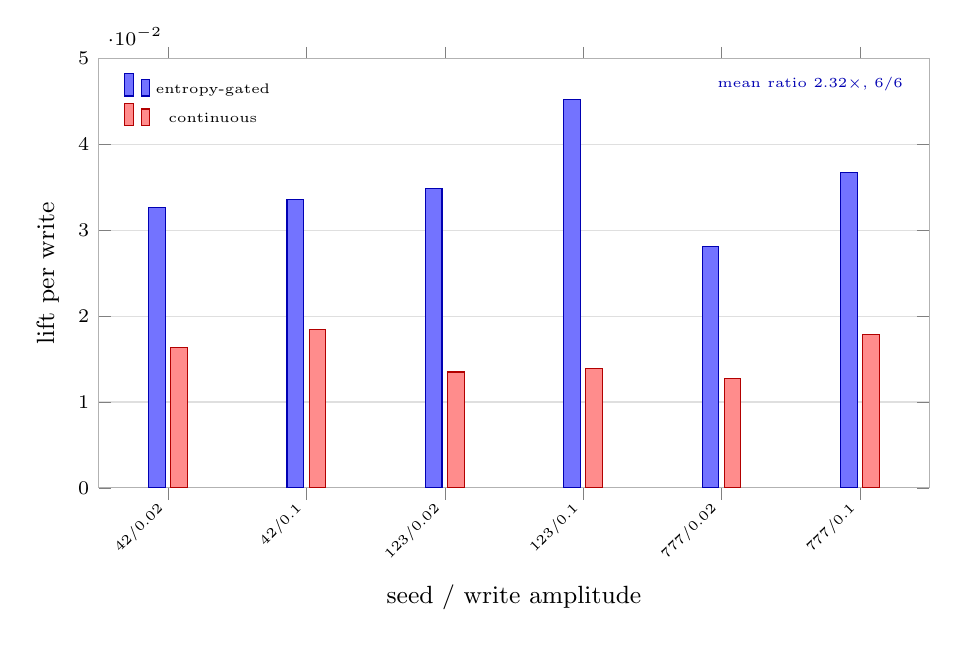
\begin{tikzpicture}
\begin{axis}[
  ybar, /pgf/bar width=6pt,
  width=\columnwidth, height=0.58\columnwidth,
  symbolic x coords={42/0.02,42/0.1,123/0.02,123/0.1,777/0.02,777/0.1},
  xtick=data, x tick label style={rotate=45, anchor=east, font=\tiny},
  xlabel={seed / write amplitude}, xlabel style={font=\scriptsize},
  ymin=0, ymax=0.05, ylabel={lift per write},
  label style={font=\small}, tick label style={font=\scriptsize},
  legend style={font=\tiny, at={(0.02,0.98)}, anchor=north west, draw=none, fill=none},
  ymajorgrids, grid style={gray!25}, axis line style={gray!60},
]
\addplot+[fill=blue!55, draw=blue!70!black] coordinates {(42/0.02,0.0327) (42/0.1,0.0336) (123/0.02,0.0349) (123/0.1,0.0452) (777/0.02,0.0281) (777/0.1,0.0367)};
\addplot+[fill=red!45, draw=red!70!black] coordinates {(42/0.02,0.0164) (42/0.1,0.0184) (123/0.02,0.0135) (123/0.1,0.0139) (777/0.02,0.0127) (777/0.1,0.0179)};
\addlegendentry{entropy-gated}
\addlegendentry{continuous}
\node[font=\tiny, blue!70!black, anchor=north east] at (rel axis cs:0.98,0.98)
  {mean ratio 2.32$\times$, 6/6};
\end{axis}
\end{tikzpicture}
}
\caption{Lift per write, entropy-gated against continuous, across six seed-by-amplitude cells (gate L22 efficiency block). Gated placement wins every cell; mean ratio 2.32, recovering roughly two-thirds of the lift at under one-third of the writes.}
\label{fig:efficiency}
\end{figure}

\subsection{F12: Recognition-Gated Hardening Is a Deployable Moat on Some Models, Predicted Before Deployment}
\label{sec:results:moat}

The activation signal that fails as a blanket steering direction (F9) succeeds when it is used the way the doctrine's verification clause suggests, as a recognition test on the input rather than an unconditional write. A defence built on the fused attacker-defender loop (external refusal-direction extraction supplied by the companion \emph{prayoga} attack library, injected through prabodha's entropy-gated writer and, in the final form, conditioned on an input-projection recognition gate) hardens a model against jailbreaks only when the input's projection onto the refusal direction crosses a threshold placed in a clean gap between benign and attack projections. On Gemma-2-2B the benign and attack projection ranges are cleanly separated at read layer 13 (benign $[-53,-18]$, attack $[+4,+73]$); placing the threshold in that gap cuts real jailbreak attack success from 0.50 to 0.25, matching brute-force unconditional hardening, but at zero benign over-refusal, whereas the unconditional defence reaches the same 0.25 only by refusing every benign prompt (over-refusal 1.00), which is unusable (gate L26 proof, exploratory, $n=12$ attacks and 10 benign, single seed).

Generality is bounded and, importantly, predictable. Across four model families the moat works on exactly two, and the predictor is the clean-gap test computed before any deployment (Figure~\ref{fig:moat}, Figure~\ref{fig:cleangap}; Table~\ref{tab:moat}). Gemma-2-2B (0.50 to 0.25) and Llama-3.2-1B (0.25 to 0.083) have cleanly separated projection ranges and harden at zero benign over-refusal. Qwen2.5-1.5B and SmolLM2-1.7B have overlapping ranges: on the former the gate cannot discriminate and attack success is unchanged while over-refusal rises, and on the latter the underlying difference-in-means direction is not a clean refusal direction, so unconditional hardening raises attack success from 0.583 to 0.917. The operational consequence is that the same read-layer projection statistic that decides whether to fire the gate at inference time also predicts, offline and cheaply, whether the moat will hold for a given model, so a deployer can test before trusting. These results are exploratory (small samples, single seed, refusal-phrase attack metric), and they are reported as an existence-and-predictability result rather than a general guarantee.

\begin{table}[t]
\caption{Recognition-gated hardening across four model families (moat consolidation, from the released \texttt{moat\_models.json}). ASR is jailbreak attack success rate; OR is benign over-refusal. The clean-gap column is the offline predictor.}
\label{tab:moat}
\vskip 0.1in
\centering
{\footnotesize
\begin{tabular}{lccccc}
\toprule
\multirow{2}{*}{\textbf{Model}} & \textbf{Clean} & \textbf{ASR} & \multicolumn{2}{c}{\textbf{Recognition-gated}} & \multirow{2}{*}{\textbf{Moat}} \\
 & \textbf{gap} & \textbf{none} & \textbf{ASR} & \textbf{OR} & \\
\midrule
Gemma-2-2B    & yes & 0.500 & 0.250 & 0.00 & works \\
Llama-3.2-1B  & yes & 0.250 & 0.083 & 0.00 & works \\
Qwen2.5-1.5B  & no  & 0.333 & 0.333 & 0.20 & fails \\
SmolLM2-1.7B  & no  & 0.583 & 0.917 & 0.00 & backfires \\
\bottomrule
\end{tabular}}
\end{table}

\begin{figure}[t]
\centering
\resizebox{\columnwidth}{!}{% Auto-generated from committed gate JSONs by generate_figures.py. Do not edit by hand.

\begin{tikzpicture}
\begin{groupplot}[
  group style={group size=2 by 1, horizontal sep=30pt},
  width=0.56\columnwidth, height=0.6\columnwidth,
  ybar, /pgf/bar width=4pt,
  symbolic x coords={Gemma-2-2B,Llama-3.2-1B,Qwen2.5-1.5B,SmolLM2-1.7B},
  xtick=data, x tick label style={rotate=40, anchor=east, font=\tiny},
  label style={font=\scriptsize}, tick label style={font=\scriptsize},
  ymajorgrids, grid style={gray!25}, axis line style={gray!60},
]
\nextgroupplot[ylabel={attack success rate}, ymin=0, ymax=1.0,
  legend style={font=\tiny, at={(0.02,0.98)}, anchor=north west, draw=none, fill=none}]
\addplot+[fill=gray!45, draw=gray!60] coordinates {(Gemma-2-2B,0.5) (Llama-3.2-1B,0.25) (Qwen2.5-1.5B,0.333) (SmolLM2-1.7B,0.583)};
\addplot+[fill=orange!55, draw=orange!70!black] coordinates {(Gemma-2-2B,0.25) (Llama-3.2-1B,0.083) (Qwen2.5-1.5B,0.25) (SmolLM2-1.7B,0.917)};
\addplot+[fill=blue!55, draw=blue!70!black] coordinates {(Gemma-2-2B,0.25) (Llama-3.2-1B,0.083) (Qwen2.5-1.5B,0.333) (SmolLM2-1.7B,0.917)};
\addlegendentry{no defence}
\addlegendentry{unconditional}
\addlegendentry{recognition-gated}
\nextgroupplot[ylabel={benign over-refusal}, ymin=0, ymax=1.05,
  legend style={font=\tiny, at={(0.02,0.98)}, anchor=north west, draw=none, fill=none}]
\addplot+[fill=orange!55, draw=orange!70!black] coordinates {(Gemma-2-2B,1.0) (Llama-3.2-1B,0.6) (Qwen2.5-1.5B,1.0) (SmolLM2-1.7B,0.0)};
\addplot+[fill=blue!55, draw=blue!70!black] coordinates {(Gemma-2-2B,0.0) (Llama-3.2-1B,0.0) (Qwen2.5-1.5B,0.2) (SmolLM2-1.7B,0.0)};
\addlegendentry{unconditional}
\addlegendentry{recognition-gated}
\end{groupplot}
\end{tikzpicture}
}
\caption{Four-model recognition-gated hardening (moat consolidation). Left: jailbreak attack success under no defence, unconditional hardening, and recognition-gated hardening. Right: benign over-refusal. Recognition gating matches the unconditional attack-success reduction where the moat holds, at a fraction of the over-refusal cost.}
\label{fig:moat}
\end{figure}

\begin{figure}[t]
\centering
\resizebox{\columnwidth}{!}{% Auto-generated from committed gate JSONs by generate_figures.py. Do not edit by hand.

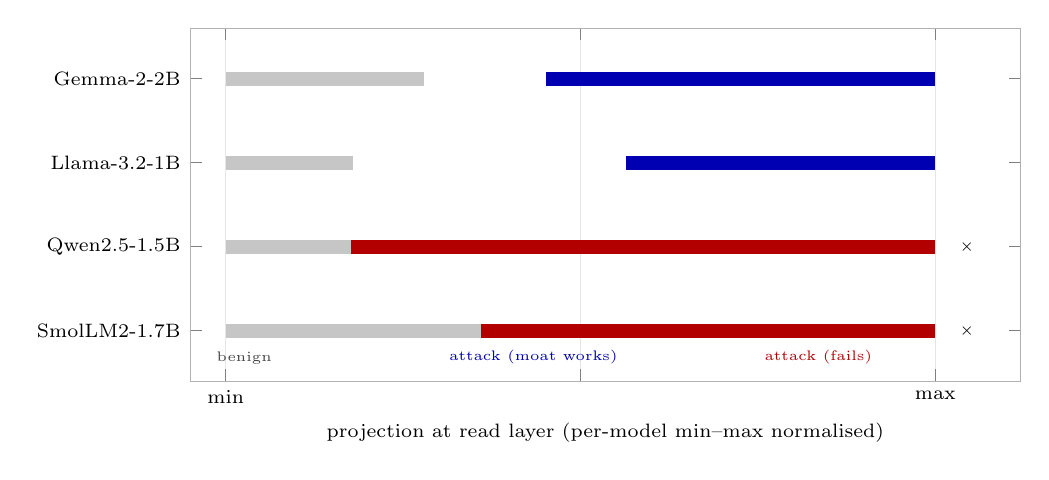
\begin{tikzpicture}
\begin{axis}[
  width=\columnwidth, height=0.5\columnwidth,
  xmin=-0.05, xmax=1.12, ymin=0.4, ymax=4.6,
  xlabel={projection at read layer (per-model min--max normalised)},
  xtick={0,0.5,1}, xticklabels={min,,max},
  ytick={4,3,2,1}, yticklabels={Gemma-2-2B,Llama-3.2-1B,Qwen2.5-1.5B,SmolLM2-1.7B},
  label style={font=\scriptsize}, tick label style={font=\scriptsize},
  axis line style={gray!60}, xmajorgrids, grid style={gray!20},
]
\addplot[draw=none] coordinates {(0,1)};
\draw[line width=5pt, gray!45] (axis cs:0.000,4) -- (axis cs:0.280,4);
\draw[line width=5pt, blue!70!black] (axis cs:0.452,4) -- (axis cs:1.000,4);
\node[font=\tiny, anchor=west] at (axis cs:1.02,4) {\checkmark};
\draw[line width=5pt, gray!45] (axis cs:0.000,3) -- (axis cs:0.179,3);
\draw[line width=5pt, blue!70!black] (axis cs:0.564,3) -- (axis cs:1.000,3);
\node[font=\tiny, anchor=west] at (axis cs:1.02,3) {\checkmark};
\draw[line width=5pt, gray!45] (axis cs:0.000,2) -- (axis cs:0.405,2);
\draw[line width=5pt, red!70!black] (axis cs:0.176,2) -- (axis cs:1.000,2);
\node[font=\tiny, anchor=west] at (axis cs:1.02,2) {$\times$};
\draw[line width=5pt, gray!45] (axis cs:0.000,1) -- (axis cs:0.447,1);
\draw[line width=5pt, red!70!black] (axis cs:0.360,1) -- (axis cs:1.000,1);
\node[font=\tiny, anchor=west] at (axis cs:1.02,1) {$\times$};
\node[font=\tiny, gray!55!black, anchor=south west] at (rel axis cs:0.02,0.02) {benign};
\node[font=\tiny, blue!70!black, anchor=south west] at (rel axis cs:0.30,0.02) {attack (moat works)};
\node[font=\tiny, red!70!black, anchor=south west] at (rel axis cs:0.68,0.02) {attack (fails)};
\end{axis}
\end{tikzpicture}
}
\caption{The clean-gap predictor. Benign (grey) and attack (coloured) projection ranges at each model's read layer, normalised per model. Separation predicts the moat: Gemma-2-2B and Llama-3.2-1B separate cleanly and harden; Qwen2.5-1.5B and SmolLM2-1.7B overlap and fail.}
\label{fig:cleangap}
\end{figure}

The hardening loop was also characterised at the activation level directly. Both Qwen3-4B and Nemotron-Mini-4B are prompt-robust but activation-vulnerable: prompt-only jailbreaks fail entirely (attack success 0.00) while activation-level refusal ablation succeeds (0.90 on Qwen3-4B, 1.00 on Nemotron-Mini-4B), which locates the harmful signature in the residual stream rather than the prompt and motivates an activation-level, rather than prompt-level, defence (gates \texttt{char}). An earlier form of the harden loop that added the direction unconditionally under entropy gating preserved freedom and cut writes (11.8 against 50 per generation) but did not resist an activation-level attacker (gate L23, registered fail), which is precisely the negative that drove the design toward input-conditioned recognition (Figure~\ref{fig:harden}).

\begin{figure}[t]
\centering
\resizebox{\columnwidth}{!}{% Auto-generated from committed gate JSONs by generate_figures.py. Do not edit by hand.

\begin{tikzpicture}
\begin{groupplot}[
  group style={group size=2 by 1, horizontal sep=30pt},
  width=0.56\columnwidth, height=0.58\columnwidth,
  ybar, /pgf/bar width=6pt,
  symbolic x coords={{baseline},{attacked},{harden\\naive},{harden\\gated}},
  xtick=data, x tick label style={align=center, font=\tiny},
  label style={font=\scriptsize}, tick label style={font=\scriptsize},
  ymajorgrids, grid style={gray!25}, axis line style={gray!60},
]
\nextgroupplot[ymin=0, ymax=1.0, ylabel={rate},
  legend style={font=\tiny, at={(0.02,0.98)}, anchor=north west, draw=none, fill=none}]
\addplot+[fill=red!50, draw=red!70!black] coordinates {({baseline},0.0) ({attacked},0.9) ({harden\\naive},0.0) ({harden\\gated},0.0)};
\addplot+[fill=orange!45, draw=orange!70!black] coordinates {({baseline},0.0) ({attacked},0.0) ({harden\\naive},0.6) ({harden\\gated},0.5)};
\addlegendentry{attack success}
\addlegendentry{benign over-refusal}
\nextgroupplot[ymin=0, ymax=55, ylabel={writes per generation}]
\addplot+[fill=blue!55, draw=blue!70!black] coordinates {({baseline},0.0) ({attacked},0.0) ({harden\\naive},50.0) ({harden\\gated},11.8)};
\end{groupplot}
\end{tikzpicture}
}
\caption{The fused attacker-defender harden loop (gate L23). Left: attack success and benign over-refusal per arm; entropy-gated hardening matches naive hardening on benign generations while using far fewer writes (right), but neither resists an activation-level attacker, motivating the recognition gate of F12.}
\label{fig:harden}
\end{figure}
